%=============================================================================
%   About pentominos
%   Reporte de pentominos - Brief Summary
%   Servicio social - Laura Natalia Borbolla Palacios
%=============================================================================

\subsection{Pentominos}
% Hey, there! We are talking about pentominos. Basic structures and how
% Conway used them to find basic configurations in the elemental automata.
For more information, please consult \cite{language-and-automata-journal, life-wiki, rit-people}.

A polyomino is a finite collection of orthogonally connected cells; or, in
another workds, a collection of equally-sized squares that form a connected
piece, meaning that each square can reach any other in it by going through
adjacent squares; the order of a polyomino is the number of squares used to
make it, so a fifth order polyomino (made of five squares), is called
pentomino. Both terms, polyomino and pentomino were first used by S. Golomb in
1953, in a talk to the Harvard Mathematics Club and a year later in an article.
There are twelve distinct pentominoes (see
Figure~\ref{fig:conway_pentominoes}) and two naming conventions, in
this paper the Conway convention (using letters \textit{O} through \textit{Z})
will be used; although the resemblance to the letters with this labeling scheme
seems a little more strained with the other scheme, specially when using the
\textit{O} instead of \textit{I}, it has the advantage that uses 12
consecutive letters; also, the Conway scheme tends to be used when discussing
topics related to cellular automata.

\begin{figure}[H]
	\centering
	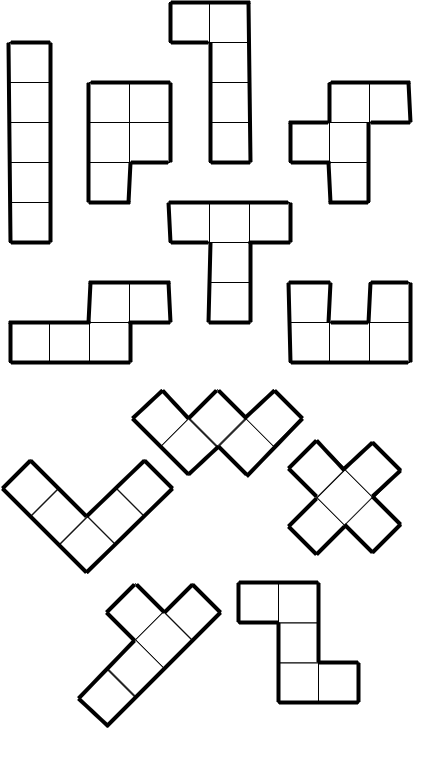
\includegraphics[scale=0.35]{diagrams/conway_pentominoes.PNG}
	\caption{Conway pentominoes from O through Z (left to right).}
  \label{fig:conway_pentominoes}
\end{figure}

%% http://www.conwaylife.com/wiki/Polyomino
%% https://books.google.com.mx/books?id=dBW6BQAAQBAJ&pg=PA16&dq=pentominos+conway&hl=es-419&sa=X&ved=0ahUKEwjl2O3qi4DgAhXnmq0KHZH3DvsQ6AEILzAB#v=onepage&q=pentominos%20conway&f=true

\subsubsection{R-Pentomino}
